\section{Zielsetzung}
\label{sec:Zielsetzung}
In diesem Versuch sollen die grundlegenden Gesetzmäßigkeiten -Relfexion, Beugung und Brechung- der klassischen Optik überprüft werden.

\section{Theorie}
\label{sec:Theorie}

\subsection{Strahlenoptik}
\label{sec:Strahlenoptik}
Die Ausbreitung von Wellen wird in der Strahlenoptik, die auch geometrische Optik genannt wird, durch die Wellennormale beschrieben.
Trifft ein Lichtstrahl nun auf eine Grenzfläche, so wird dieser gebrochen. Durch die Materialabhängigkeit der Lichtgeschwindigkeit im
Medium, durch den der Lichtstrahl läuft, können die Ausbreitungsgeschwindigkeiten $v_{\symup{1}}$ und $v_{\symup{2}}$ durch die
Brechungsindizes $n_{\symup{1}}$ und $n_{\symup{2}}$ der Materialien und durch den Einfallswinkel $\alpha$ und den Brechungswinkel
$\beta$ durch die Gleichung
\begin{align*}
    \frac{sin\,\alpha}{sin\,\beta} = \frac{v_{\symup{1}}}{v_{\symup{2}}} = \frac{n_{\symup{2}}}{\symup{1}}
\end{align*}
beschrieben werden. In diesem Versuch ist das eine Medium Luft, das die Ausbreitungsgeschwindigkeit $v_{\symup{1}} = 22,9979 \cdot
10^{8}\,\unit{\meter\per\second}$ und einen Brechungsindex von $n_{\symup{1}} = 1,000292$ hat \cite{sample}. Da der Lichtstrahl 
immer von Glas auf Luft, in der die Lichtgeschwindigkeit größer ist, trifft, ist Luft das optische dünnere Medium und Glas das
optisch dichtere Medium.

\subsubsection{Reflexion}
\label{sec:Reflexion}
Nach dem Reflexionsgesetz ist Einfallswinkel gleich Ausfallswinkel. Dementsprechend gilt
\begin{align}
    \label{eqn:Reflexion}
    \alpha_{\symup{1}} = \alpha_{\symup{2}}.
\end{align}

\subsubsection{Brechung}
\label{sec:Brechung}
Wenn ein Lichtstrahl mit Einfallswinkel $\alpha$ auf ein anderes Medium mit Brechungsindx $n$ trifft,
erfährt er eine Richtungsänderung. Dieser Umstand wird Brechung genannt und lässt sich durch das Snelliussche 
Brechungsgesetz
\begin{align}
    \label{eqn:Snellius}
    n_{\symup{1}}sin\,\alpha = n_{\symup{2}}sin\,\beta
\end{align}
beschreiben. $\beta$ ist dabei der Ausfallswinkel.

\subsubsection{Reflexion und Transmission}
\label{sec:Reflexion_und_Transmission}
Im den meisten Fällen tritt Reflexion und Brechung gleichzeitig auf, wenn Licht auf ein anderes Medium trifft. So wird ein
Teil des Lichts reflektiert und ein anderer transmissiert und gebrochen. Das Verhältnis von reflektierten und transmissierten
Licht ist material abhängig, aber für die Intensitäten muss gelten $R + T = 1$.\\
\\
In \autoref{fig:skizzen} sind die oben genannten Gesetze noch einmal graphisch dargestellt.
\begin{figure}
    \begin{subfigure}{0.3\textwidth}
        \centering
        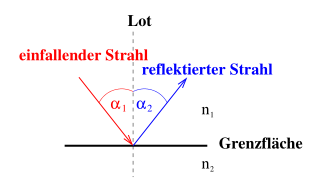
\includegraphics{Bilder/Reflexion.png}
        \caption{Reflexion.}
        \label{fig:Reflexion}
    \end{subfigure}
    \hfill
    \begin{subfigure}{0.3\textwidth}
        \centering
        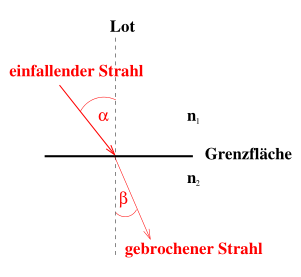
\includegraphics{Bilder/Brechung.png}
        \caption{Brechung.}
        \label{fig:Brechung}
    \end{subfigure}
    \hfill
    \begin{subfigure}{0.3\textwidth}
        \centering
        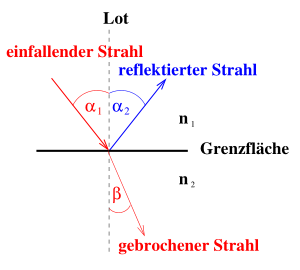
\includegraphics{Bilder/Transmission.png}
        \caption{Transmission.}
        \label{fig:Transmission}
    \end{subfigure}
    \caption{Skizzen von Reflexion, Brechung und Transmission.}
    \label{fig:skizzen}
\end{figure}

\subsection{Wellenoptik}
\label{sec:Wellenoptik}
Sobald Licht auf Objekte trifft, die verhältnismäßig klein im Vergleich zur Wellenlänge sind, kommt die geometrische Optik an ihre
Grenzen, da sich nun das Licht auch im Schattenraum ausbreitet.